\documentclass[10pt,oneside]{article}

\usepackage[T1]{fontenc}

\usepackage[paper=a4paper,margin=2cm,bottom=2.5cm]{geometry}
\usepackage[sfdefault,light,condensed]{roboto}
\usepackage[export]{adjustbox}
\usepackage[usenames,dvipsnames,table]{xcolor}

\usepackage{amsmath,amssymb,array,fancyhdr,graphicx,enumitem,lastpage,listings,lstautogobble,multicol,tabularx,textcomp,titlesec}
\usepackage{mathtools}

\setlength\parindent{0cm}
\renewcommand\headrule{}
\setlength{\footskip}{1.25cm}


\pagestyle{fancy}

\usepackage{fontawesome,subcaption,tikzsymbols}

% Add some padding to all table cells.
\setlength\extrarowheight{1pt}

%\newcommand{\boxwidth}{\dimexpr\linewidth - 2pt}
\newcommand{\boxwidth}{\linewidth}

\definecolor{BoxHeaderBG}{RGB}{50, 50, 50}
\definecolor{BoxHeaderText}{RGB}{220, 220, 220}

\definecolor{QuestionHeaderBG}{RGB}{200, 200, 200}
\definecolor{QuestionHeaderText}{RGB}{0, 0, 0}

\newcommand{\BoxHeader}[2]{
    \multicolumn{#1}{| >{\bfseries\footnotesize\cellcolor{BoxHeaderBG}\arraybackslash}l |}{
        \textcolor{BoxHeaderText}{#2}
    }
}

\newcounter{QuestionCounter}

\newcommand{\Question}[2]{
    \stepcounter{QuestionCounter}
    \begin{tabularx}{\boxwidth}{|X|}
        \hline
        \cellcolor{QuestionHeaderBG}{\footnotesize\bfseries \textcolor{QuestionHeaderText}{Question \#\theQuestionCounter}} {\em \textcolor{QuestionHeaderText}{#1}} \\\hline
        \ \\[#2]\hline
    \end{tabularx}

    \medskip
}

\newcommand{\FeelQuestion}{
    \stepcounter{QuestionCounter}
    \newcolumntype{F}{>{\centering\arraybackslash}X}
    \begin{tabularx}{\boxwidth}{| F F F |}
        \hline
        \multicolumn{3}{| >{\hsize=\dimexpr3\hsize+4\tabcolsep+2\arrayrulewidth\relax}X |}{
            \cellcolor{QuestionHeaderBG}{\footnotesize\bfseries \textcolor{QuestionHeaderText}{Question \#\theQuestionCounter}} {\em \textcolor{QuestionHeaderText}{Select the option which best reflects how confident you are in applying what you have learend in this lesson.}}}\\\hline
        & & \\[-8pt]
        \Sadey[5][orange] & \Neutrey[5][gray] & \Smiley[5][cyan] \\\hline
    \end{tabularx}

    \medskip
}

\lhead{\tiny\texttt{U\UnitNumber: \UnitTitle\\L\LessonNumber: \LessonTitle}}
\rhead{\tiny\texttt{[DPCS/\CourseLevel/U\UnitNumber/\LessonNumber]\\ }}

\lfoot{
\includegraphics[height=2cm,valign=c]{Files/logo}}
\cfoot{\footnotesize \LessonTitle/DPCS/\CourseLevel/U\UnitNumber/L\LessonNumber/\thepage/\pageref{LastPage}\\Woodstock School/Mussoorie, Uttarakhand, India}
\rfoot{
\includegraphics[height=2cm,valign=c]{Files/ib-world-school-logo-1-colour}}


\def\CourseLevel{SL}

\def\UnitNumber{01}
\def\UnitTitle{The Computer}

\def\LessonNumber{03}
\def\LessonTitle{The Machine Instruction Cycle}

\begin{document}
    %Lesson Title
    \begin{center}
        \Large\bfseries \LessonTitle
    \end{center}

    % Objectives List
    \begin{tabularx}{\boxwidth}{|>{\small\raggedleft\bfseries\arraybackslash}p{0.1\textwidth} >{\small\arraybackslash}X |}
        \hline
        \BoxHeader{2}{Objectives} \\\hline
        2.1.4 & Explain the machine instruction cycle. \\\hline
    \end{tabularx}

    % Opening Exercise
    \section*{Before You Begin}
    The following diagram represents a \emph{procedural abstraction} of the \emph{Machine Instruction Cycle}. This is the process by which a computer system reads and executes commands within its CPU.

    \begin{figure}[h]
        \centering
        \definecolor{NodeBG}{RGB}{180,180,220}
        \begin{tikzpicture}[scale=1.5]
            \huge
            \draw[very thick,->,>=triangle 45] (90:4cm and 2cm) arc (90:-15:4cm and 2cm);
            \draw[very thick,->,>=triangle 45] (-30:4cm and 2cm) arc (-30:-133:4cm and 2cm);
            \draw[very thick,->,>=triangle 45] (-150:4cm and 2cm) arc (-150:-258:4cm and 2cm);
            \node[fill=NodeBG,draw,rounded corners = 0.25cm] at (90:4cm and 2cm) {Fetch};
            \node[fill=NodeBG,draw,rounded corners = 0.25cm] at (210:4cm and 2cm) {Execute};
            \node[fill=NodeBG,draw,rounded corners = 0.25cm] at (330:4cm and 2cm) {Decode};
            %\draw (0, 0) ellipse (4cm and 2cm);
        \end{tikzpicture}
        \caption{A broad overview of the machine instruction cycle.}
    \end{figure}

    Based on your knowledge of the core components of a computer system from our previosu lessons, which part of the CPU do you believe handles each step of the cycle?

    \medskip
    \begin{tabularx}{\boxwidth}{| >{\em\arraybackslash}p{0.25\boxwidth} | p{0.25\boxwidth} | X |}
        \hline
        \BoxHeader{1}{Step} & \BoxHeader{1}{Component} & \BoxHeader{1}{Justification} \\\hline
        Fetch Instruction & & \\[1cm]\hline
        Decode Instruction & & \\[1cm]\hline
        Execute Instruction & & \\[1cm]\hline
    \end{tabularx}

    \vfill

    \Question{An abstraction such as the one shown here is known as a \emph{high-level abstraction} because it hides almost all of the complexity of a system in favour of being human readable. What are the benefits and drawbacks to such a high level of abstraction?}{4cm}

    \pagebreak
    
    % Definitions
    \section*{Important Terms}
    \begin{tabularx}{\boxwidth}{| >{\bfseries\arraybackslash}p{0.3\textwidth} | X | }
        \hline
        \BoxHeader{1}{Term} & \BoxHeader{1}{Definition} \\\hline
        Current Instruction Register (CIR) & \\[2cm]\hline
        Instructino & \\[2cm]\hline
        Interrupt & \\[2cm]\hline
        Jump & \\[2cm]\hline
        Program Counter (PC) & \\[2cm]\hline
    \end{tabularx}

    \pagebreak

    % Technical Background
    \section*{Technical Background}

    \subsection*{Fetching Instructions}
    The following flow chart represents a lower-level abstraction of the fetch phase of the instruction cycle.

    \begin{figure}[h]
        \centering
        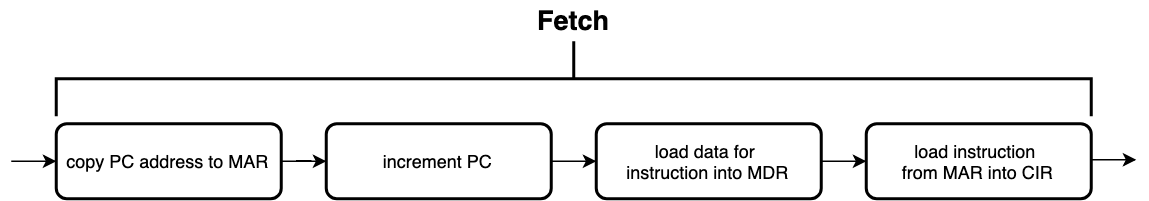
\includegraphics[width=0.9\boxwidth]{Extras/cycle_fetch}
        \caption{A closer look at the fetch part of the machine instruction cycle.}
    \end{figure}

    \subsubsection*{Notes}

    \vfill

    \Question{The final process in the fetch phase of the machine instruction cycle loads the instruction from the address in one register (MAR) into another (CIR). What benefit to the overall cycle does the use of a second register have?}{4cm}

    \pagebreak
    
    \subsection*{The Fetch-Decode-Execute (FDX) Cycle}
    The following flowchart shows the entire FDX (\textbf{F}etch-\textbf{D}ecode-E\textbf{x}eute) cycle, including special decisions in the case of a jump instruction and the presence of interrupts.

    \begin{figure}[h]
        \centering
        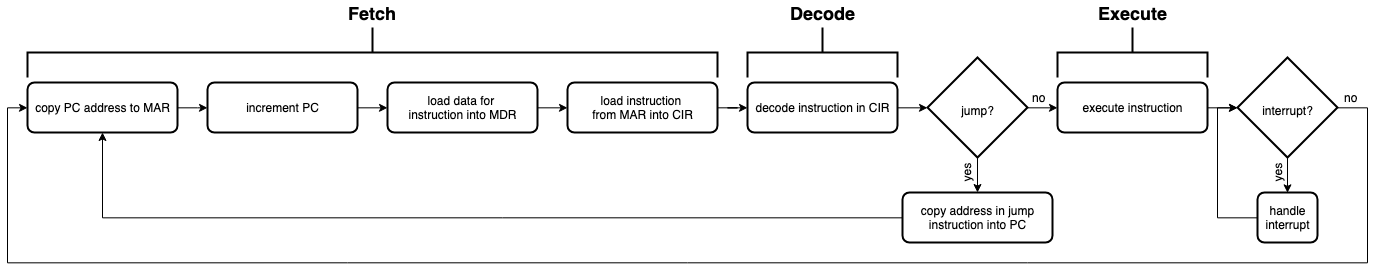
\includegraphics[width=0.9\boxwidth]{Extras/cycle_fdx}
        \caption{A look at the entire machine instruction cycle.}
    \end{figure}

    \subsubsection*{Notes}

    \vfill

    \Question{Why do you think interrupts are handled as a special step in the machine instruction cycle, rather than simply being added to the instruction queue?}{4cm}

    \pagebreak
    
    \subsection*{Sample Instruction Set}
    The following table shows the first ten instructions available in the popular ``x86 Instruction Set'' (likely the instruction set being used by your own personal computer's processor).

    \smallskip
    {\small{\textbf{Note:} Repeated instruction names are listed as each operation code (``opcode'') refers to instructions manipulating data in different memory locations and registers, which is beyond the scope of this course.}

    \medskip
    \newcolumntype{C}{>{\centering\arraybackslash}X}
    \begin{tabularx}{\boxwidth}{| C | C | C | C | C | C | C | C | C | C |}
        \hline
        00 & 01 & 02 & 03 & 04 & 05 & 06 & 07 & 08 & 09 \\\hline
        \multicolumn{6}{| c |}{ADD} & PUSH & POP & \multicolumn{2}{| c |}{OR} \\\hline
    \end{tabularx}

    \medskip
    More information about this and related instruction sets are avialalbe through Intel's website:\\
    https://software.intel.com/en-us/articles/intel-sdm.

    \subsubsection*{Notes}

    \vfill

    \Question{Although the 8086 processor was first published by Intel in 1974, most of its core instruction set is still in use with more modern Intel and compatible processors. Why is maintaining consistency and ``backwards compatibility'' despite advances in technology important for the computing and software industries?}{4cm}

    \pagebreak
    
    % Developing Technical Skills
    \section*{Developing Technical Skills}
    \subsubsection*{Assembly Language Programming}
    Along with the instruction set, the x86 specification also provides the description of an ``aseembly language''. This family of languages is a very low-level language designed to interact almost directly with the instruction.

    \medskip
    In this activity, you'll be looking at a simple assembly language program and adding comments to each line of code. Relevant descriptions of assembly language syntax and commands are given below.

    \medskip
    \begin{tabularx}{\boxwidth}{| p{0.2\boxwidth} | X |}
        \hline
        \BoxHeader{1}{Syntax} & \BoxHeader{1}{Description} \\\hline
        \emph{ax, bx, etc...} & Reference to specific 16-bit data registers provided automatically by the system. \\\hline
        \emph{ah, bh, etc...} / \emph{al, bl, etc...} & Reference to the ``highest''/``lowest'' 8-bits of each data register provided automatically by the system.\\\hline
        \textbf{ADD} A, B & Add the data from B into register A. \\\hline
        A \textbf{DW} B & Create a data word named ``A'' and store the value B. \\\hline
        \textbf{END MAIN} & Denotes the end of the program. \\\hline
        A \textbf{ENDP} & Ends the description of a specific procedure named ``A''. \\\hline
        \textbf{INT 21H} & Call an interrupt to the MS-DOS API interrupt table. \\
        & {\small Note: the MS-DOS API specifies interrupt ``02'' as callilng for character output.} \\\hline
        \textbf{MOV} A, B & Copy data from B into register A. \\\hline
        A \textbf{PROC} & Start the description of a specific procedure named ``A''.\\\hline
    \end{tabularx}

    \medskip
    Add a comment next to each of the following lines of code based on the syntax description above. A few comments have already been made for you.

    \smallskip
    {\small Note \#1: Comments in x86 assembly are separated from the text of the program using a \texttt{;} character.}\\
    {\small Note \#2: Numbers appended with an ``H'' denote hexadecimal values.}

    \bigskip
    {
        \renewcommand\arraystretch{1.25}
        \begin{tabularx}{\boxwidth}{| >{\ttfamily}c | >{\ttfamily}l >{\ttfamily}X |}
            \BoxHeader{1}{\#} & \BoxHeader{1}{Code} & \BoxHeader{1}{Comment} \\\hline
            01 & .stack 100H & ; set aside 256 bits of memory for the program. \\
            02 & & \\
            03 & .data & ; begin the data section of the program \\
            04 & a DW 02H & \\
            05 & b DW 03H & \\
            06 & & \\
            07 & .code & ; begin the code section of the program \\
            08 & MAIN PROC & \\
            09 & MOV ax, @data & \\
            10 & MOV ds, ax & \\
            11 & & \\
            12 & MOV ax, a & \\
            13 & MOV bx, b & \\
            14 & & \\
            15 & ADD ax, bx & \\
            16 & & \\
            17 & MOV ah, 02 & \\
            18 & MOV dx, ax & \\
            19 & INT 21H & \\
            20 & & \\
            21 & MAIN ENDP & \\
            22 & END MAIN & \\\hline
        \end{tabularx}
    }

    \pagebreak

    % Reflections
    \section*{Reflections}

    \Question{In January 2006, Apple began producing a line of their Macintosh computers using the now-standard Intell processor. Previously, they had been using the Apple-IBM-Motorola produced PowerPC line of processors. What impact do you think this switch, along with its change in instruction set, had on software development for Apple computers?}{4cm}

    \Question{The processors used by many mobile devices use the ARM architecture, which implements a Reduced Instruction Set Computer (RISC). What benefits and drawbacks does implementing a less complex instruction set in a processor provide?}{4cm}

    \Question{Describe at least one new thing you have learned from this lesson. How might you apply this knowledge in the future?}{4cm}

    \FeelQuestion

    \Question{What further questions do you still have about this lesson's content?}{4cm}
\end{document}